\documentclass[tikz,border=3pt]{standalone}
\usepackage{amsmath}
\usepackage{xcolor}
\usetikzlibrary{arrows.meta,positioning,calc}

\definecolor{ink}{HTML}{17202A}
\definecolor{muted}{HTML}{5D6D7E}
\definecolor{blue}{HTML}{1F77B4}
\definecolor{cyan}{HTML}{17A2B8}
\definecolor{green}{HTML}{2E7D32}
\definecolor{orange}{HTML}{E67E22}
\definecolor{red}{HTML}{C0392B}
\definecolor{violet}{HTML}{6C5CE7}
\definecolor{line}{HTML}{B8C2CC}

\tikzset{
  font=\sffamily,
  panel/.style={rounded corners=3pt, draw=line, line width=0.8pt, fill=white},
  box/.style={rounded corners=3pt, draw=#1, line width=0.9pt, fill=#1!8, align=center, inner xsep=5pt, inner ysep=5pt, minimum height=9mm},
  smallbox/.style={rounded corners=2pt, draw=#1, line width=0.75pt, fill=#1!7, align=center, inner xsep=4pt, inner ysep=4pt, minimum height=7mm},
  arrow/.style={-{Latex[length=2.1mm,width=1.7mm]}, line width=0.85pt, draw=ink},
  feedback/.style={-{Latex[length=2.1mm,width=1.7mm]}, line width=0.85pt, draw=violet, dashed},
  stage/.style={font=\sffamily\bfseries\footnotesize, text=ink},
  note/.style={font=\sffamily\scriptsize, text=muted, align=center}
}

\begin{document}
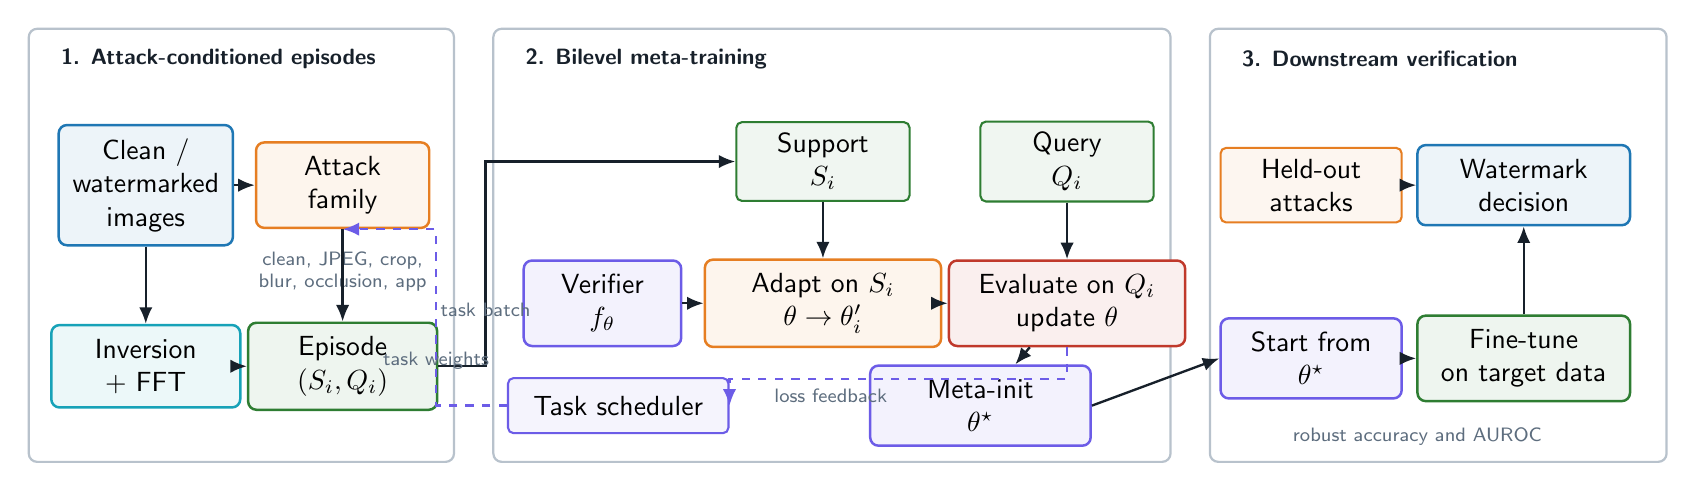
\begin{tikzpicture}[x=1mm,y=1mm]

% Panels
\node[panel, minimum width=54mm, minimum height=55mm, anchor=north west] (p1) at (0,0) {};
\node[panel, minimum width=86mm, minimum height=55mm, anchor=north west] (p2) at (59,0) {};
\node[panel, minimum width=58mm, minimum height=55mm, anchor=north west] (p3) at (150,0) {};

\node[stage, anchor=west] at ($(p1.north west)+(3,-4)$) {1. Attack-conditioned episodes};
\node[stage, anchor=west] at ($(p2.north west)+(3,-4)$) {2. Bilevel meta-training};
\node[stage, anchor=west] at ($(p3.north west)+(3,-4)$) {3. Downstream verification};

% Stage 1
\node[box=blue, minimum width=21mm] (imgs) at (15,-20) {Clean /\\watermarked\\images};
\node[box=orange, minimum width=22mm] (pool) at (40,-20) {Attack\\family};
\node[note] at (40,-31) {clean, JPEG, crop,\\blur, occlusion, app};
\node[box=cyan, minimum width=24mm] (features) at (15,-43) {Inversion\\+ FFT};
\node[box=green, minimum width=24mm] (episode) at (40,-43) {Episode\\$(S_i,Q_i)$};

\draw[arrow] (imgs) -- (pool);
\draw[arrow] (imgs.south) -- (features.north);
\draw[arrow] (pool.south) -- (episode.north);
\draw[arrow] (features) -- (episode);

% Stage 2
\node[box=violet, minimum width=20mm] (theta) at (73,-35) {Verifier\\$f_\theta$};
\node[smallbox=green, minimum width=22mm] (support) at (101,-17) {Support\\$S_i$};
\node[smallbox=green, minimum width=22mm] (query) at (132,-17) {Query\\$Q_i$};
\node[box=orange, minimum width=30mm] (adapt) at (101,-35) {Adapt on $S_i$\\$\theta \rightarrow \theta'_i$};
\node[box=red, minimum width=30mm] (outer) at (132,-35) {Evaluate on $Q_i$\\update $\theta$};
\node[smallbox=violet, minimum width=28mm] (scheduler) at (75,-48) {Task scheduler};
\node[box=violet, minimum width=28mm] (metainit) at (121,-48) {Meta-init\\$\theta^\star$};

\draw[arrow] (episode.east) -- ++(6,0) |- node[pos=0.18, below, note] {task batch} (support.west);
\draw[arrow] (theta) -- (adapt);
\draw[arrow] (support) -- (adapt);
\draw[arrow] (query) -- (outer);
\draw[arrow] (adapt) -- (outer);
\draw[arrow] (outer) -- (metainit);
\draw[feedback] (outer.south) -- ++(0,-4) -| node[pos=0.35, below, note] {loss feedback} (scheduler.east);
\draw[feedback] (scheduler.west) -- ++(-9,0) |- node[pos=0.18, below, note] {task weights} (pool.south);

% Stage 3
\node[smallbox=orange, minimum width=23mm] (heldout) at (163,-20) {Held-out\\attacks};
\node[box=blue, minimum width=27mm] (decision) at (190,-20) {Watermark\\decision};
\node[box=violet, minimum width=23mm] (init) at (163,-42) {Start from\\$\theta^\star$};
\node[box=green, minimum width=27mm] (fine) at (190,-42) {Fine-tune\\on target data};
\node[note] at (176.5,-52) {robust accuracy and AUROC};

\draw[arrow] (metainit.east) -- (init.west);
\draw[arrow] (init) -- (fine);
\draw[arrow] (fine.north) -- (decision.south);
\draw[arrow] (heldout) -- (decision);

\end{tikzpicture}
\end{document}
